\documentclass[lualatex,aspectratio=169]{beamer}

\usepackage[utf8]{inputenc}
\usepackage[T1]{fontenc}
\usepackage{xspace}
\usepackage{graphicx}

\graphicspath{ {./images/} }

\title{Accelerating $k$-D Trees for Nearest Neighbor Search on Walk-on-Spheres}
\date[\today]{\today}
\author[Ryan Smith]{Ryan Smith}


\newcommand{\kd}{$k$-D\xspace}

\usetheme{NIST}

\begin{document}

\begin{frame}
  \titlepage
\end{frame}

\begin{frame} 

  \frametitle{Outline} 
  %\framesubtitle{The proof uses \textit{reductio ad absurdum}.} 

  \begin{itemize} 
    \item Motivation and specification
    \item Introduction to \kd trees
    \item Limitations of \kd trees
    \item Flattened \kd trees
    \item Implementation details
    \item Performance results
    \item Areas for improvement
  \end{itemize}

\end{frame}


\begin{frame}
  \frametitle{Motivation}
  \framesubtitle{ZENO/Walk-on-Spheres}

  \begin{itemize}
    \item ZENO/Walk-on-Spheres is an accelerated implementation of the ZENO computation which is a Monte Carlo
      numerical path integration that yields material properties such as:
    \begin{itemize}
      \item electrostatic capacity
      \item polarizability tensor
      \item intrinsic conductivity 
      \item hydrodynamic radius
      \item translational diffusion constant
      \item and more
    \end{itemize}
  \end{itemize}

\end{frame}

\begin{frame}
  \frametitle{Motivation}
  \framesubtitle{ZENO/Walk-on-Spheres}

  \begin{figure}
    \centering
    \includegraphics[width=0.7\textwidth]{80000_NOBGCROP.png}
    \caption{DNA-grafted gold nano-particles interacting with a 
    two-dimensional DNA-based origami construct (23115 speheres).}
    \label{fig:80000}
  \end{figure}
\end{frame}

\begin{frame}
  \frametitle{Motivation}
  \framesubtitle{ZENO/Walk-on-Spheres}

  \begin{columns}[T]
    \begin{column}{.5\textwidth}
      \begin{block}{}%
        {\color{white} Walk-on-Spheres accelerates Brownian Motion by jumping %
          to a uniformly distributed point on the surface of a surrounding sphere}
      \end{block}
    \end{column}
    \begin{column}{.5\textwidth}
      \begin{block}{}
        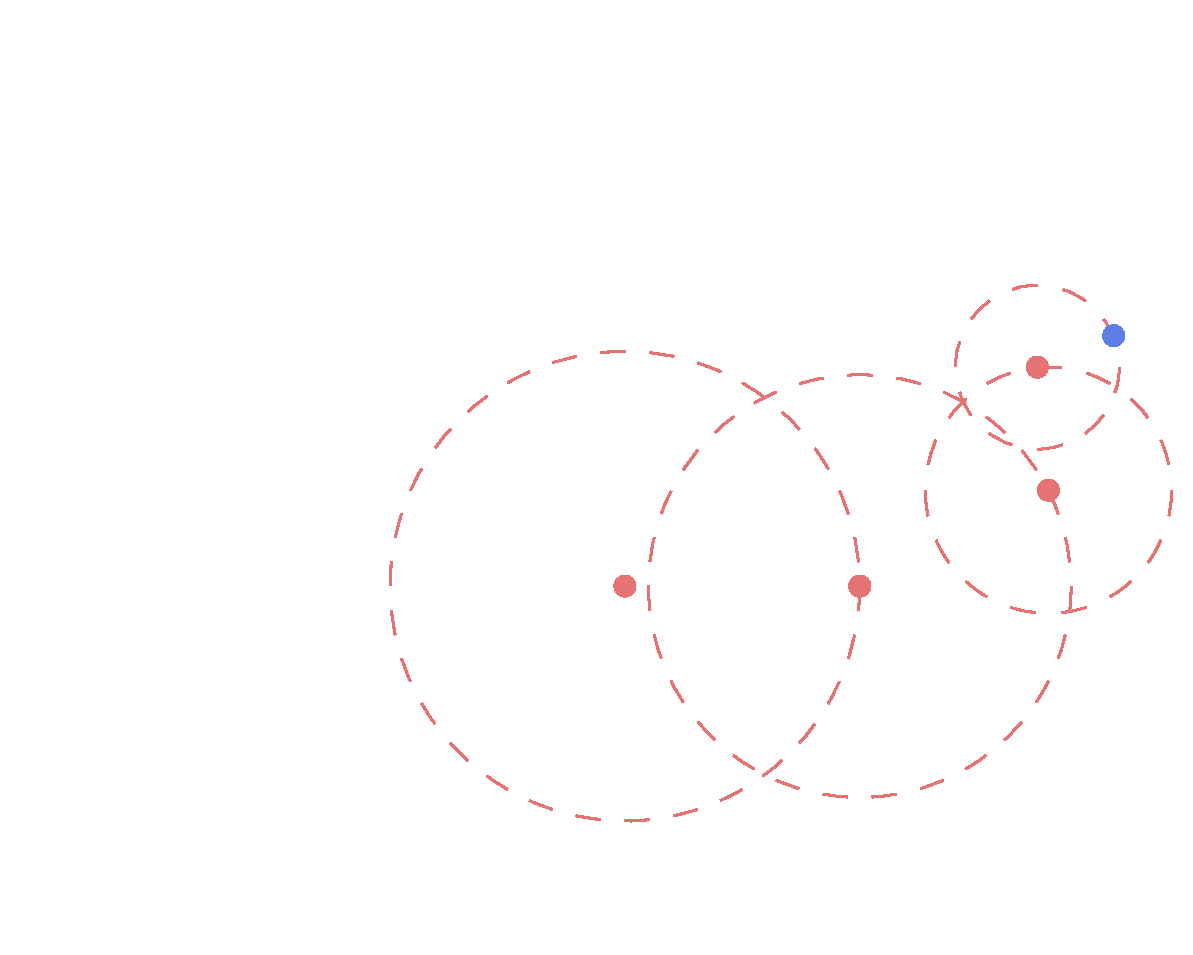
\includegraphics[width=\textwidth]{WoS.pdf}
      \end{block}
    \end{column}
  \end{columns}
\end{frame}

\begin{frame}
  \frametitle{Specification}

  {\usebeamerfont{title}\color{white}
  Improve performance of nearest neighbor search on \kd trees by more compactly organizing tree components
  to reduce cache misses and load instructions.}

\end{frame}



%%%%%%%%%%%%%%%%%%%%%%%%%%%%%%%%%%%%%%%%
%             Background               %
%%%%%%%%%%%%%%%%%%%%%%%%%%%%%%%%%%%%%%%%

\begin{frame}
  \frametitle{\kd trees}
  \framesubtitle{Introduction}

  \begin{itemize}
    \item A \kd tree is a data structure used for partitioning $k$-dimensional space
    \item At each node, a cluster of points is partitioned by a hyperplane and the resulting
      sets of points contained in the half-spaces are passed down to the child nodes
    \item Often, hyperplanes are kept orthogonal to one coordinate axis of the space
    \item Binary search trees are the one-dimensional versions of \kd trees
  \end{itemize}

\end{frame}

\begin{frame}
  \frametitle{\kd trees}
  \framesubtitle{Example: $k=1$}
  
  Graphic of binary search tree here
  
\end{frame}

\begin{frame}
  \frametitle{\kd trees}
  \framesubtitle{Example: $k=2$}
  
  Graphic of 2-d tree
  Maybe show a sequence of tree construction 
  
\end{frame}

\begin{frame}
  \frametitle{\kd trees}
  \framesubtitle{Example: $k=3$}
  
  Graphic of 3-d tree
  
\end{frame}

\begin{frame}
  \frametitle{\kd trees}
  \framesubtitle{Nearest neighbor search}

  \begin{enumerate}
    \item Given a point, $p$, rescursively move down the tree by computing the points orientation relative to the 
      hyperplane $t$ given by $p - \text{proj}_t(p)$
    \item At each node, compare the distance of the query point to the node's splitting point with the distance
      of the current nearest neighbor, if smaller, update nearest neighbor candidate
    \item Upon completion of recursive call, compare the distance of current nearest neighbor 
      candidate to the point with the distance to the hyperplane $\|p - \text{proj}_t(p)\|$; 
      if it is larger, search the other child branch of the node
  \end{enumerate}

\end{frame}

\begin{frame}
  \frametitle{\kd trees}
  \framesubtitle{Nanoflann}

  \begin{itemize}
    \item Header-only C++ \kd tree implementation that supports k-nearest neighbor and radius search with 
      L1 or L2 metric
    \item Utilizes curiously recurring template pattern and inlined functions for high performance
    \item Used for nearest neighbor search in our ZENO/Walk-on-Spheres implementation 
  \end{itemize}

\end{frame}

%%%%%%%%%%%%%%%%%%%%%%%%%%%%%%%%%%%%%%%%
%             Limitations              %
%%%%%%%%%%%%%%%%%%%%%%%%%%%%%%%%%%%%%%%%

\begin{frame}
  \frametitle{\kd trees}
  \framesubtitle{Limitations of trees}

  \begin{itemize}
    \item Access pattern of memory when searching tree is unpredictable - difficult to prefetch memory
    \item Spatially close points can end up far away in the tree (e.g., neighboring points divided by 
      root's hyperplane)
  \end{itemize}
\end{frame}

\begin{frame}
  \frametitle{\kd trees}
  \framesubtitle{Height and its memory limitations}

  \begin{itemize}
    \item In the best case, when the tree is balanced, the height is $O(\log n)$
    \item Each search query will require at least $O(\log n )$ pointer dereferences - very costly on graphics 
      hardware
    \item At each node we can only look ahead to one additional subspace of points
  \end{itemize}
\end{frame}

\begin{frame}
  \frametitle{\kd trees}
  \framesubtitle{Height and its memory limitations}

  \begin{itemize}
    \item Costly edge cases lead to large variance in search dereferences and time
  \end{itemize}

  Insert image showing edge case when we would have to traverse both large sides of tree
\end{frame}



\end{document}
